\chapter{Simulation Model}
\label{ch:orbital}

The fitness $J$ of Chapter~\ref{ch:method} is computed by a mission simulation, the
\emph{engine}. Given a feasible design it propagates every spacecraft, turns its positions into
the rotating asteroid frame, decides which facets it photographs at each step, and tracks its
battery. All sizes, speeds and times are kept at their real values (Figure~\ref{fig:hero}).

\begin{figure}[htbp]
\centering
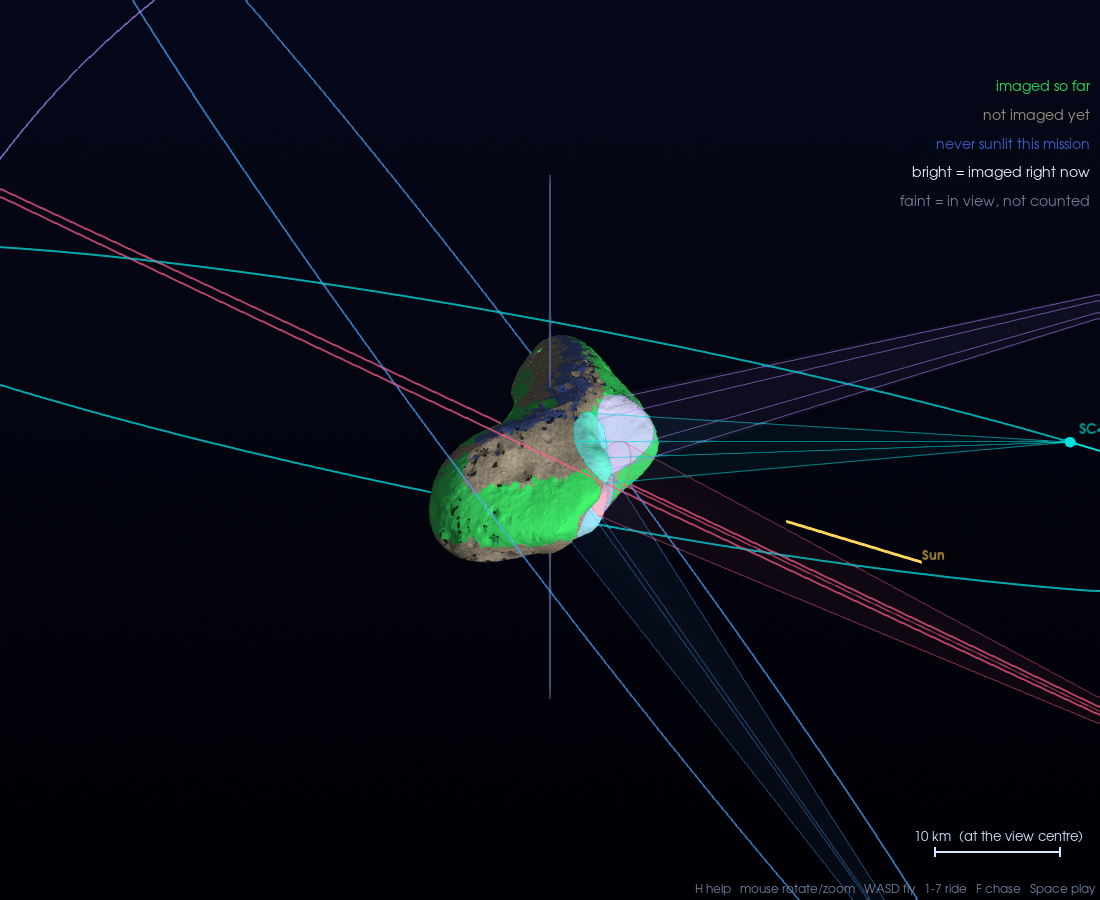
\includegraphics[width=0.7\textwidth]{Figures/hero.png}
\caption{The simulator at true scale: the best design of case A2 (four spacecraft, Eros) after
4.4\,h, with the orbits and the $6^\circ$ camera cones; green facets are already photographed,
dark blue facets are never sunlit during the mission, the yellow line points to the Sun.}
\label{fig:hero}
\end{figure}

\section{Asteroid mesh}
The surface is a triangle mesh (Figure~\ref{fig:mesh}). Facet $f$ has area $A_f$, centre
$\mathbf{c}_f$ and outward unit normal $\mathbf{n}_f$, all in the body frame $B$ that spins with the
asteroid. Eros uses NASA's Gaskell shape model~\cite{gaskell2008} (49\,152 facets, from NEAR Shoemaker images)
decimated to 1\,500 facets for the search; every final design is re-checked on a 6\,000-facet
copy (validation V7). Kleopatra uses the radar shape model of Ostro et al.~\cite{ostro2000} (4\,092 facets),
shifted to its centre of mass.

\begin{figure}[htbp]
\centering
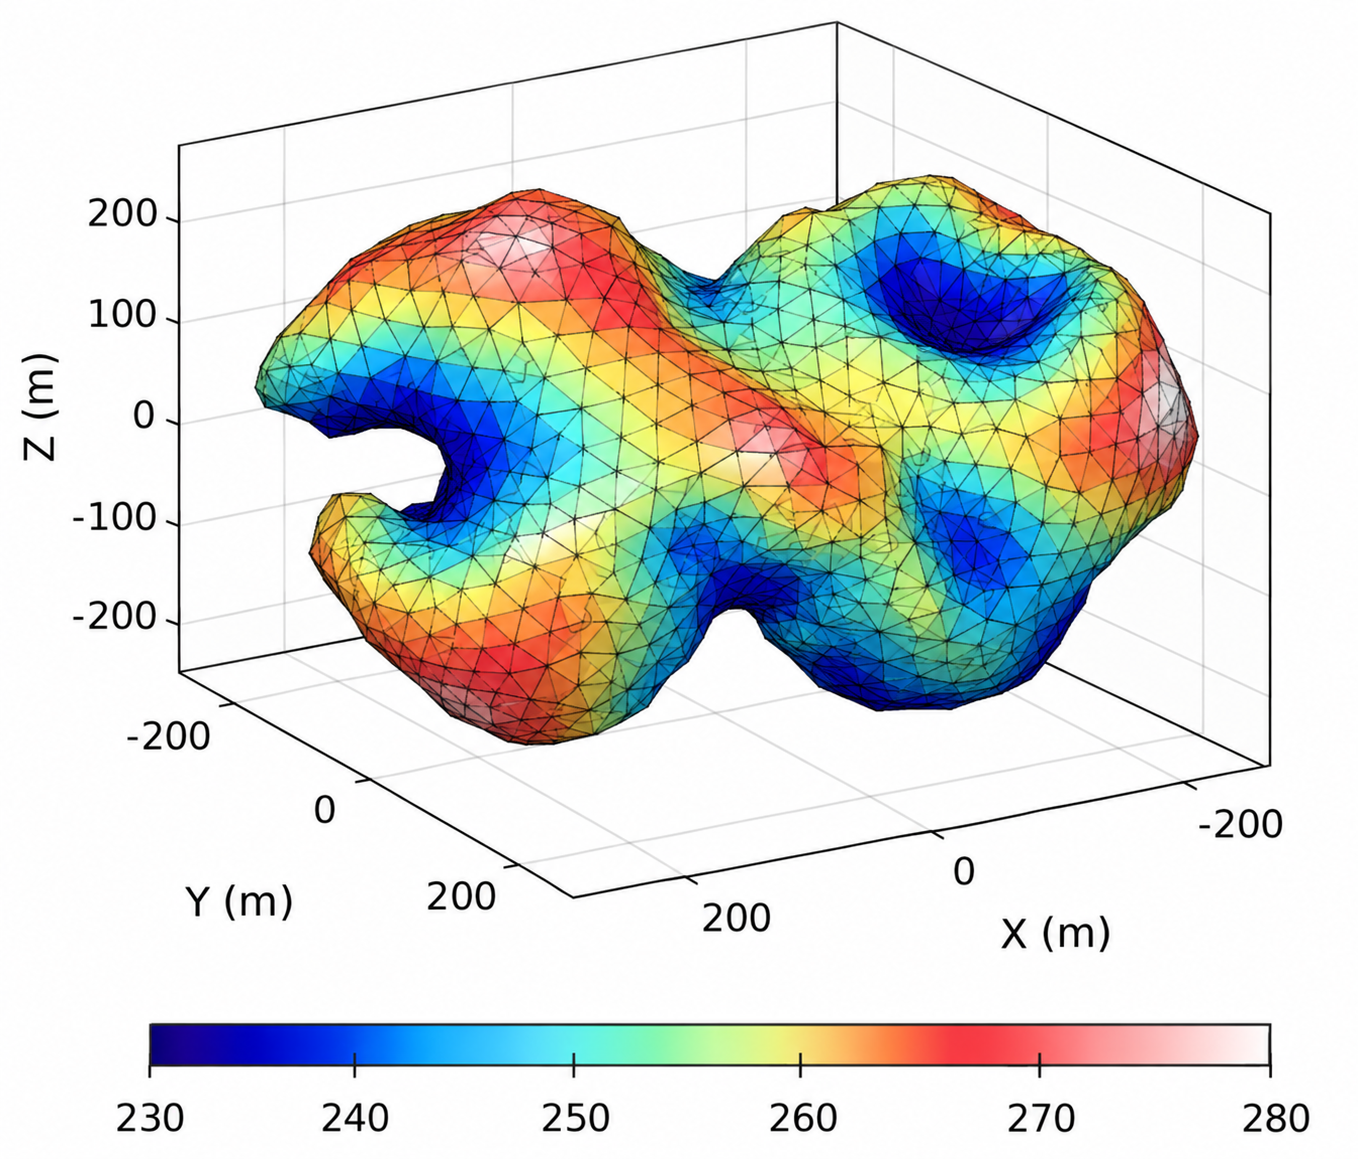
\includegraphics[width=0.55\textwidth]{Figures/mesh_example.png}
\caption{The asteroid as a triangle mesh: every facet is one small flat piece of the surface.}
\label{fig:mesh}
\end{figure}

\section{Stage 1: orbit propagation}
For a circular orbit of radius $a_i$ the spacecraft moves at the constant mean motion
\begin{equation}
n_i=\sqrt{\mu/a_i^{3}},\qquad u_i(t)=M_{0,i}+n_i\,t ,
\end{equation}
where $u_i$ is the angle travelled along the orbit from the ascending node. Its inertial position
is the in-plane point turned into place by the node and the inclination:
\begin{equation}
\mathbf{r}^{I}_i(t)=R_3(-\Omega_i)\,R_1(-\iota_i)\,\bigl[a_i\cos u_i(t),\;a_i\sin u_i(t),\;0\bigr]^{T},
\end{equation}
with $R_1$, $R_3$ the elementary rotations about the $x$ and $z$ axes. (The code propagates
general Kepler ellipses with a Newton solver of Kepler's equation; with $e=0$ it reduces to the
above.) For Eros at $a=35$\,km the period is $2\pi/n=17.1$\,h, while Eros turns once every
5.27\,h, so the surface slides beneath every orbit.

\section{Stage 2: rotation into the asteroid frame}
Instead of rotating the mesh at every step, each spacecraft position is rotated into the spinning
body frame:
\begin{equation}
\mathbf{r}^{B}_i(t)=R_z(\omega_{\mathrm{ast}}t)^{T}\,\mathbf{r}^{I}_i(t),\qquad
\omega_{\mathrm{ast}}=2\pi/P_{\mathrm{rot}} .
\end{equation}

\section{Stage 3: which facets are photographed}
\label{sec:visibility}
For spacecraft $i$ at step $k$ let $\mathbf{r}=\mathbf{r}^{B}_i(t_k)$,
$\mathbf{q}=\mathbf{r}-\mathbf{c}_f$ (facet to spacecraft), $\ell=\|\mathbf{q}\|$,
$\hat{\mathbf{q}}=\mathbf{q}/\ell$ and $\hat{\mathbf{b}}=-\mathbf{r}/\|\mathbf{r}\|$ (nadir
boresight). Facet $f$ is photographed with usable quality, $V_{ifk}=1$, only if all five tests
hold:
\begin{align}
&\text{(a) inside the camera cone:} && \hat{\mathbf{b}}\cdot(-\hat{\mathbf{q}})\ge\cos(\psi/2)\\
&\text{(b) not too oblique:} && \mathbf{n}_f\cdot\hat{\mathbf{q}}\ge\cos\eta_{\max}\\
&\text{(c) line of sight free:} && \text{the ray from }\mathbf{c}_f\text{ towards }\mathbf{r}\text{ hits no other facet}\\
&\text{(d) sharp enough:} && \mathrm{GSD}=\frac{2\,\ell\tan(\psi/2)}{p}\le\mathrm{GSD}_{\max}
 \iff \ell\le\ell_{\max}=\frac{\mathrm{GSD}_{\max}\,p}{2\tan(\psi/2)}\\
&\text{(e) sunlit:} && \mathbf{n}_f\cdot\hat{\mathbf{s}}(t_k)\ge\cos 70^\circ\text{ and the ray from }\mathbf{c}_f\\
&&&\text{towards the Sun hits no other facet}
\end{align}
$\hat{\mathbf{s}}(t_k)$ is the Sun direction in the body frame. Test (c) and the shadow part of
(e) cast rays with the M\"oller--Trumbore intersection test~\cite{moller1997}, accelerated with
Embree through \texttt{trimesh}. The cheap tests (d), (a), (b), (e) are applied first, and only the
surviving facet--step pairs are ray-cast. The lighting test (e) does not depend on the design, so
it is computed once per case study; it also defines $A^{*}$ in~(\ref{eq:C}).

The observations are then combined over time and across the fleet:
\begin{equation}
v_{if}=\max_{k:\,t_k\le T}V_{ifk},\qquad u_f=\max_i v_{if},\qquad
n_{\mathrm{img},i}=\#\{k:\,t_k\le T,\ \textstyle\sum_f V_{ifk}>0\}.
\end{equation}

\section{Stage 4: $\Delta V$, power and battery}
\label{sec:dv}
\textbf{$\Delta V$.} From the circular equatorial arrival orbit $r_0$, a spacecraft first tilts its
plane, then transfers to radius $a_i$ with a Hohmann transfer:
\begin{equation}
\Delta V_i=2v_0\sin\frac{\iota_i}{2}
+\Bigl|\sqrt{\mu\Bigl(\tfrac{2}{r_0}-\tfrac{1}{a_t}\Bigr)}-v_0\Bigr|
+\Bigl|\sqrt{\tfrac{\mu}{a_i}}-\sqrt{\mu\Bigl(\tfrac{2}{a_i}-\tfrac{1}{a_t}\Bigr)}\Bigr|,
\qquad a_t=\frac{r_0+a_i}{2}.
\end{equation}
For Eros $v_0=3.0$\,m/s, so a polar orbit costs about 4.2\,m/s for the plane change alone.

\textbf{Eclipses and battery.} A spacecraft is in eclipse when it is behind the asteroid (a sphere
of the body's mean radius) as seen from the Sun. Its battery (200\,Wh, starting full) is updated
every step:
\begin{equation}
Q_i(t_{k+1})=\min\Bigl\{Q_{\mathrm{cap}},\;Q_i(t_k)+\Delta t\,\bigl[P_{\mathrm{sol}}\,(1-\epsilon_{ik})-P_{\mathrm{base}}
-\delta_{ik}\,\tfrac{e_{\mathrm{img}}+e_{\mathrm{tx}}}{\Delta t}\bigr]\Bigr\},\qquad q_i(t_k)=\frac{Q_i(t_k)}{Q_{\mathrm{cap}}},
\end{equation}
where $\epsilon_{ik}=1$ in eclipse and $\delta_{ik}=1$ when a frame is taken. The lowest $q_i$ enters
constraint $g_4$.

\section{Making the simulation fast enough}
One evaluation simulates $N$ spacecraft over up to $N_t=T_{\max}/\Delta t+1$ steps (1\,441 for
ten days) against every facet. Two design decisions keep the cost manageable:
\begin{itemize}
\item \textbf{Per-spacecraft tracks.} Everything in stages 1--4 depends only on one spacecraft's
own orbit. The engine therefore simulates each spacecraft separately over the whole horizon
$T_{\max}$ and caches the result (its \emph{track}) under its four orbit variables. A design of
duration $T$ simply uses the steps $t_k\le T$ of its tracks. Changing $T$ or switching a slot on
or off therefore costs no new simulation, and moving one orbit costs one track.
\item \textbf{Vectorised geometry.} Tests (a), (b) and (d) need only the products
$\mathbf{r}\cdot\mathbf{c}_f$ and $\mathbf{r}\cdot\mathbf{n}_f$, so a block of steps is two matrix
products instead of a loop over facets.
\end{itemize}
